% ============================================================
%  part5/ch30-observer-horizons.tex
%  Chapter 30: Observer Horizons
% ============================================================

\chapter{Observer Horizons}
\label{ch:observer-horizons}

\epigraph{%
  The observer never sees the whole.\\
  The next chapter asks whether the whole\\
  can nevertheless be reconstructed.%
}{---}

\begin{WhyChapter}
  Chapter~\ref{ch:horizons} introduced horizons intuitively.
  Chapter~\ref{ch:sheaf} introduced the full sheaf machinery.
  This chapter occupies the space between them: it formalises
  Oculara, overlap compatibility, and presheaf structure,
  and motivates cohomological obstruction without yet
  introducing the full machinery.
  The reader who finishes this chapter is prepared for the
  Monoturn (Chapter~\ref{ch:monoturn}) and the cohomological
  results of Chapter~\ref{ch:sheaf}.
\end{WhyChapter}


\begin{ChapterIntro}
Every observer occupies a limited position within a larger reality.

Some limitations are practical. Others are fundamental. Distance, scale, causality, bandwidth, memory, and finite observation all impose boundaries on what can be known directly.

A horizon is not merely a barrier. It is a filter. It determines which distinctions are visible and which become indistinguishable. Different observers therefore inhabit different observational worlds even when they occupy the same physical universe.

The challenge is not simply understanding what an observer sees. It is understanding what can be inferred about the larger structure from what remains visible.
\end{ChapterIntro}

\section{Oculara}

\begin{definition}[Ocularum]
  \label{def:ocularum-formal}
  The \emph{Ocularum} of observer $O_i$ is the structured
  observational domain
  \[
    \mathcal{O}_i = (H_i, \mathcal{A}(H_i), \pi_i),
  \]
  where:
  \begin{itemize}[leftmargin=2em]
    \item $H_i \subseteq X$ is the accessible region
      (causal horizon, instrument aperture, etc.),
    \item $\mathcal{A}(H_i)$ is the space of admissible local
      field configurations over $H_i$,
    \item $\pi_i : \mathcal{A}(H_i) \to O_{\mathrm{obs}}^{(i)}$
      is the projection into observable states.
  \end{itemize}
\end{definition}

\begin{proposition}[Horizon access is a projection]
  \label{prop:horizon-projection}
  \statusproven{}
  If $H_i \subsetneq X$, then $F_i : X \to \mathcal{A}(H_i)$
  is non-injective.
\end{proposition}

\begin{proof}
  Since $H_i \subsetneq X$, there exists $p \in X \setminus H_i$.
  Two global configurations differing only outside $H_i$ produce
  identical local data.
  Therefore $F_i$ is non-injective.
\end{proof}

\section{Observable sections and restriction maps}

\begin{definition}[Observable section]
  An \emph{observable section} for observer $O_i$ is any
  $s_i \in \mathcal{A}(H_i)$.
  It is the admissible field configuration consistent with
  $O_i$'s observations.
\end{definition}

\begin{definition}[Restriction map]
  For $H_j \subseteq H_i$, the restriction map
  $\rho^{H_i}_{H_j} : \mathcal{A}(H_i) \to \mathcal{A}(H_j)$
  sends $s_i \mapsto s_i|_{H_j}$.
\end{definition}

\begin{proposition}[Restriction maps compose]
  \label{prop:restriction-compose}
  \statusproven{}
  For $H_k \subseteq H_j \subseteq H_i$:
  $\rho^{H_j}_{H_k} \circ \rho^{H_i}_{H_j} = \rho^{H_i}_{H_k}$.
\end{proposition}

\begin{proof}
  $(s_i|_{H_j})|_{H_k} = s_i|_{H_k}$ by the transitivity
  of restriction.
\end{proof}

\section{Overlap compatibility}

When two observers share overlapping horizons, their observable
sections must agree on the overlap for a consistent global
picture to exist.

\begin{definition}[Overlap region]
  $H_{ij} = H_i \cap H_j$.
\end{definition}

\begin{definition}[Compatible sections]
  Sections $s_i \in \mathcal{A}(H_i)$ and
  $s_j \in \mathcal{A}(H_j)$ are \emph{compatible} if
  \[
    s_i|_{H_{ij}} = s_j|_{H_{ij}}.
  \]
\end{definition}

\begin{proposition}[Compatible overlaps define a presheaf]
  \label{prop:presheaf-horizons}
  \statusproven{}
  The assignment $H_i \mapsto \mathcal{A}(H_i)$ with
  restriction maps $\rho^{H_i}_{H_j}$ is a presheaf.
\end{proposition}

\begin{proof}
  (1) Identity: $\rho^{H_i}_{H_i}(s_i) = s_i|_{H_i} = s_i$.
  (2) Composition: $\rho^{H_j}_{H_k} \circ \rho^{H_i}_{H_j}
  = \rho^{H_i}_{H_k}$ by Proposition~\ref{prop:restriction-compose}.
  These are exactly the presheaf axioms.
\end{proof}

\section{Multiple observers and overlap discrepancy}

\begin{definition}[Overlap discrepancy]
  \label{def:overlap-discrepancy}
  \[
    D_{ij} = \|s_i|_{H_{ij}} - s_j|_{H_{ij}}\|_{H^k(H_{ij})}.
  \]
\end{definition}

\begin{definition}[Total obstruction measure]
  \label{def:total-obstruction}
  \[
    \mathcal{O} = \sum_{i,j} D_{ij}^2.
  \]
\end{definition}

\begin{proposition}[Zero obstruction $\Leftrightarrow$ compatibility]
  \label{prop:zero-obstruction}
  \statusproven{}
  $\mathcal{O} = 0$ iff all pairs $(s_i, s_j)$ are compatible.
\end{proposition}

\begin{proof}
  $\mathcal{O} = 0$ iff every $D_{ij} = 0$ iff every
  $\|s_i|_{H_{ij}} - s_j|_{H_{ij}}\|_{H^k} = 0$ iff
  $s_i|_{H_{ij}} = s_j|_{H_{ij}}$ a.e.\ for all $i,j$.
\end{proof}

\section{Mayer--Vietoris motivation}

For two observers with $X = H_1 \cup H_2$, the Mayer--Vietoris
sequence organises the obstruction:

\begin{equation}
  0
  \to \mathcal{A}(X)
  \xrightarrow{\rho_1 \oplus \rho_2}
  \mathcal{A}(H_1) \oplus \mathcal{A}(H_2)
  \xrightarrow{\delta}
  \mathcal{A}(H_{12})
  \to H^1(X, \mathcal{A})
  \to 0,
  \label{eq:mayer-vietoris}
\end{equation}
where $\delta(s_1, s_2) = s_1|_{H_{12}} - s_2|_{H_{12}}$.

\begin{theorem}[Two-observer reconstruction criterion]
  \label{thm:two-observer}
  \statusproven{}
  For $X = H_1 \cup H_2$, a global section $s \in \mathcal{A}(X)$
  exists with $s|_{H_i} = s_i$ iff $(s_1, s_2)$ is in the
  kernel of $\delta$, i.e., $D_{12} = 0$.
\end{theorem}

\begin{proof}
  Exactness of sequence~\eqref{eq:mayer-vietoris} at
  $\mathcal{A}(H_1) \oplus \mathcal{A}(H_2)$:
  $\ker\delta = \mathrm{Im}(\rho_1 \oplus \rho_2)$.
  So compatible pairs $(s_1, s_2)$ correspond exactly to
  restrictions of global sections.
  When $H^1(X,\mathcal{A}) \neq 0$, some compatible pairs
  cannot be globally reconstructed.
\end{proof}

\begin{ForwardRef}
  The Mayer--Vietoris sequence presented here motivates but
  does not yet fully develop cohomological obstruction theory.
  Chapter~\ref{ch:sheaf} develops $H^1(X,\mathcal{A})$ fully.
  Chapter~\ref{ch:monoturn} identifies the Monoturn as the
  object for which $H^1 \neq 0$ is unavoidable.
\end{ForwardRef}

\section{Bridge to the Monoturn}

The observer never sees $\mathcal{M}$; every observer sees
only their Ocularum $\mathcal{O}_i$.

\begin{proposition}[Horizon incompleteness]
  \statusproven{}
  $\mathcal{M} \neq H_i$ for every observer $O_i$.
  Hence no single observer can reconstruct $\mathcal{M}$.
\end{proposition}

\begin{proof}
  $H_i \subsetneq \mathcal{M}$ by construction.
\end{proof}

The next chapter asks: can $\mathcal{M}$ nevertheless be
reconstructed from all observers \emph{together}?
The answer depends on $H^1(\mathcal{M}, \mathcal{A})$.

\begin{ProblemSet}
\problem{
  Two observers have horizons $H_1 = [0, 2]$ and $H_2 = [1, 3]$
  on $X = [0, 3]$ with $H_{12} = [1, 2]$.
  Observer 1 measures $s_1(x) = x$ on $H_1$.
  Observer 2 measures $s_2(x) = x + 0.1$ on $H_2$.
  Compute $D_{12}$.
  Can a global section $s$ exist with $s|_{H_i} = s_i$?
}
\problem{
  Prove that the restriction map
  $\rho^U_V : \mathcal{A}(U) \to \mathcal{A}(V)$
  is well-defined for RSVP admissibility sections,
  i.e., that restricting an admissible section produces
  an admissible section.
}
\problem{
  For the Mayer--Vietoris sequence with two overlapping
  intervals $H_1 = (0,2)$, $H_2 = (1,3)$, $H_{12} = (1,2)$,
  write out the exact sequence~\eqref{eq:mayer-vietoris}
  with $\mathcal{A}(U) = C^\infty(U)$.
  What is $H^1(X, C^\infty)$ in this case?
}
\problem{
  \textbf{Conceptual problem.}
  In everyday life, two witnesses observe an event from
  different positions (different Oculara).
  Their reports are compatible on the overlap of their
  fields of view.
  (a) Formulate this as a presheaf problem.
  (b) What would a nonzero $H^1$ correspond to physically?
  (c) How does this relate to the Rashomon effect in perception?
}
\end{ProblemSet}

\section{Overlap obstruction: necessity proof}

\begin{theorem}[Overlap agreement is necessary for reconstruction]
  \label{thm:overlap-necessary}
  \statusproven{}
  Let $X = U_1 \cup U_2$ and $U_{12} = U_1 \cap U_2$.
  If a global section $s \in \mathcal{A}(X)$ exists with
  $s|_{U_i} = s_i$, then $\delta(s_1,s_2) = 0$, where
  $\delta(s_1,s_2) = s_1|_{U_{12}} - s_2|_{U_{12}}$.
\end{theorem}

\begin{proof}
  Restrict both equations $s|_{U_i} = s_i$ to $U_{12}$:
  $s_1|_{U_{12}} = s|_{U_{12}} = s_2|_{U_{12}}$.
  Therefore $\delta(s_1,s_2) = s_1|_{U_{12}} - s_2|_{U_{12}} = 0$.
\end{proof}

\begin{TechNote}[Necessity vs.\ sufficiency]
  Theorem~\ref{thm:overlap-necessary} proves necessity:
  $\delta = 0$ is required for a global section to exist.
  Sufficiency --- that $\delta = 0$ \emph{implies} a global
  section exists --- is the sheaf gluing axiom, which holds
  when $\mathcal{A}$ is a sheaf
  (Theorem~\ref{thm:unique-gluing}).
  When $\mathcal{A}$ is only a presheaf, or when the cover
  is not fine enough, compatibility is necessary but not
  sufficient.
  The obstruction to sufficiency is measured by
  $H^1(X,\mathcal{A})$.
\end{TechNote}

% ---- Figures and citations ----------------------------------

\begin{figure}[ht]
\centering
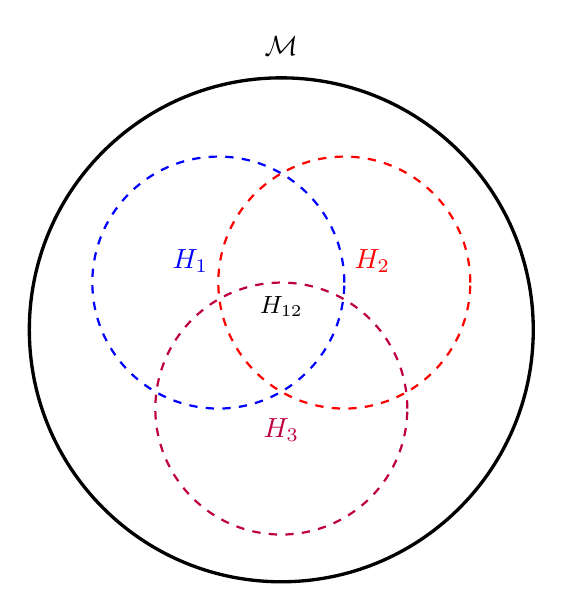
\begin{tikzpicture}
  % Monoturn (background)
  \draw[very thick] (0,0) circle (3.2);
  \node at (0,3.6) {$\mathcal{M}$};
  % Three observer horizons
  \draw[thick,blue,dashed] (-0.8,0.6) circle (1.6)
    node[above left,blue] {$H_1$};
  \draw[thick,red,dashed] (0.8,0.6) circle (1.6)
    node[above right,red] {$H_2$};
  \draw[thick,purple,dashed] (0,-1.0) circle (1.6)
    node[below,purple] {$H_3$};
  % Overlap label
  \node at (0,0.3) {\small $H_{12}$};
\end{tikzpicture}
\caption{Three overlapping observer horizons within the Monoturn
         $\mathcal{M}$.
         Each $H_i \subsetneq \mathcal{M}$ (Proposition~\ref{prop:horizon-projection}).
         Compatible sections on pairwise overlaps (Mayer--Vietoris)
         are necessary but not sufficient for global reconstruction.}
\label{fig:horizon-cover}
\end{figure}

\[
\begin{tikzcd}
  \mathcal{A}(U)
  \arrow[r,"\rho^U_{U_1} \oplus \rho^U_{U_2}"]
  &
  \mathcal{A}(U_1) \oplus \mathcal{A}(U_2)
  \arrow[r,"\delta"]
  &
  \mathcal{A}(U_{12})
  \arrow[r]
  &
  H^1(U,\mathcal{A})
\end{tikzcd}
\]

\begin{CitationAnchor}
  The presheaf and sheaf formalism (Propositions~\ref{prop:restriction-compose},~\ref{prop:presheaf-horizons})
  follows Bredon~\cite{bredon1997} and Kashiwara \& Schapira~\cite{kashiwara2006}.
  The Mayer--Vietoris sequence for sheaf cohomology is a standard
  tool; see Tennison (1975) or Mac Lane \& Moerdijk (1992) for
  an accessible treatment.
  The physical interpretation of sheaf restriction maps as
  observational constraints is an application of standard
  mathematical machinery to the observation problem.
\end{CitationAnchor}

\begin{FurtherReading}
  The theory of sheaves is developed in Bredon~\cite{bredon1997}
  (accessible) and Kashiwara \& Schapira~\cite{kashiwara2006}
  (comprehensive).
  Mac Lane \& Moerdijk's \textit{Sheaves in Geometry and Logic}
  provides the connection to topos theory.
  For sheaves in physics, see the survey by Baez \& Lauda (2011).
\end{FurtherReading}
